%%
%% sample document for AAMAS'18 conference
%%
%% modified from sample-sigconf.tex
%%
%% see ACM instructions acmguide.pdf
%%
%% AAMAS-specific questions? n.yorke-smith@tudelft.nl
%%

\documentclass[sigconf]{aamas}  % do not change this line!

%% your usepackages here, for example:
\usepackage{booktabs}

%% do not change the following lines
\setcopyright{ifaamas}  % do not change this line!
\acmDOI{doi}  % do not change this line!
\acmISBN{}  % do not change this line!
\acmConference[AAMAS'18]{Proc.\@ of the 17th International Conference on Autonomous Agents and Multiagent Systems (AAMAS 2018), M.~Dastani, G.~Sukthankar, E.~Andre, S.~Koenig (eds.)}{July 2018}{Stockholm, Sweden}  % do not change this line!
\acmYear{2018}  % do not change this line!
\copyrightyear{2018}  % do not change this line!
\acmPrice{}  % do not change this line!

%% the rest of your preamble here
\usepackage{amssymb}
%\usepackage{named}
%\setcounter{tocdepth}{3}
\usepackage{graphicx}
\usepackage{amsmath}
%\usepackage[numbers]{natbib}
\usepackage{mathtools}

\usepackage{tabularx,ragged2e}
\newcolumntype{C}{>{\Centering\arraybackslash}X} % centered "X" column

\usepackage{booktabs}
\usepackage{multirow}
\usepackage{wrapfig}
\usepackage{rotating} % <-- HERE
\usepackage{multirow}

\usepackage{tikz}
\usepackage{tikzsymbols}



\newcommand{\ET}[1]{{\textcolor{blue}{#1}}}

%%%%%%%%%%%%%%%%%%%%%%%%%%%%%%%%%%%%%%%%%%%%%%%%%%%%%%%%%%%%
\newlength{\mylengthleft}
\setlength{\mylengthleft}{1ex}
\newlength{\mylength}
\setlength{\mylength}{0.45\textwidth}
\addtolength{\mylength}{-\mylengthleft}
%%%%%%%%%%%%%%%%%%%%%%%%%%%%%%%%%%%%%%%%%%%%%%%%%%%%%%%%%%%%%%%%%%%%%%%%%%%%%%%%%%%%%%%%%%%%%%%%%%%%%%%%%

\begin{document}

%\title{Sample AAMAS Paper using the New ACM LaTeX Template}  % put your title here!
\title{Deterministic Solutions Based on Maximum Regrets in MDPs with Imprecise Rewards}
%\title{Deterministic Solutions Based on Maximum Regrets in Markov Decision Processes with Imprecise Rewards}


\begin{abstract}  % put your abstract here!
In several real world applications of sequential decision making under uncertainty a stochastic policy is not easily interpretable for the system users. This might be due to the nature of the problem or to the system requirements. In these contexts, it is more convenient (inevitable) to provide a deterministic policy to the user. In this paper, we propose an approach for computing a deterministic policy for a Markov Decision Process with Imprecise Rewards in reasonable computational overhead in comparison to the required time for computing the optimal stochastic policy. To better motivate the use of an exact procedure for finding a deterministic policy, we show some cases where the intuitive idea of using a deterministic policy obtained after ``determinising" (rounding) the optimal stochastic policy leads to a deterministic policy different from the optimal.
\end{abstract}


\keywords{Markov Decision Processes, Minimax Regret, Unknown Rewards, Deterministic Policy, Stochastic Policy}

\maketitle


%%%%%%%%%%%%%%%%%%%%%%%%%%%%%%%%%%%%%%%%%%%%%%%%%%%%%%%%%%%%%%%%%%%%%%%%%%%%%%%%%%%%%%%%%%%%%%%%%%%%%%%%%
%% start of main body of paper

\section{Introduction}


%outline for introduction
%\begin{itemize}
%\item MDP are important to model many things
%\item examples of MDP (special attention to MDP that can would prefer to have a deterministic policy)
%\item introduce concept of unknown reward
%\item mention several ways to deal with unknown reward, among them minimax regret.
%\item but the majority of the approaches proposes a stochastic policy
%\item det policy are preferable in several situation
%-- ethic \\
%-- finance \\
%\end{itemize}

Markov Decision Processes (MDPs) have proven to be effective models for representing and solving sequential decision problems under uncertainty. It is natural to model a decision-making problem in dynamic environment as an MDP. To mention just few examples: navigation, robotics or service composition problems are all well-established applications of MDPs. In navigation context such as assistant autonomous vehicles, at each stage, the agent executes an action with probabilistic effects and this state conducts her to a next state and yields a reward (penalty). The goal is to maximise the expected sum of rewards. The environment %dynamic
 (traffics and roads) is modelled as states and actions with probability assignment.%affections?. 
 
%This motivates using MDPs that account for this ambiguity in model parameters. 
 
%Despite of knowing the final goal, specifying rewards or punishments for choosing actions in states is never obvious. 
Mannor et al. \shortcite{Mannor2007} demonstrate that the strategy found via an optimisation process under the MDPs with numerical parameters, sometimes can be much worse than the anticipated policy. This can happen for multiple reasons:
%\begin{itemize}
%\item 
(1) insufficient data to estimate the rewards,
%\item 
(2) parts of models are too complex to detail, % In assistant vehicle example, defining exact rewards for all actions is time consuming or complicated and can variate during the driving process. %For this reason, we consider them bounded in real valued intervals,
%\item 
and (3) conflicting elicitations from users. %In the assistant vehicle case, if the model is designed for different drivers with various preferences, even after a limited number of communications with drivers and diminishing the rewards imprecision to a smaller sets, the MDP is not precise yet. 
%\end{itemize}

%In MDPs with unknown rewards, the system have all information about the dynamics (road and traffics) and final goal but it lacks some information about the user preferences inside the system
Several approaches have been proposed in the literature to find the best \textit{policy} (strategy) in an environment with imprecise rewards. This work is focused on the \textit{minimax regret criterion}. The basic idea is to find the policy with the minimum lost in comparison with other possible policies and reward instantiations. Minimising the max regret is more optimistic then  minimising the worst case scenario and has been widely used in the literature. %In the context of MDPs, it has been used, among others, in \cite{Regan2009,Xu2009}.

The majority of the exact and approximate methods for solving an MDP accept to have \textit{stochastic policies} as feasible policies for the MDP. A policy is defined as stochastic if, for a given state, the action to be taken is chosen with a given probability associated to each possible state.
On the other hand, in a \textit{deterministic policy}, the action to be taken in a state is uniquely defined.\\
The use of stochastic policies present two main advantages. From a algorithmic point of view (as shown also in this work), finding an optimal stochastic policy is usually easier than finding the optimal deterministic policy. Moreover, accepting also stochastic policies implies to explore a larger search space in comparison to the search space of the deterministic policies, allowing to have optimal policies with a better value than the one of an optimal deterministic policy.

Despite these two obvious advantages of stochastic over deterministic policies, in several situations the use of stochastic policies can be either not recommended or not possible. 
%
%
First of all, the use of a stochastic policy could be ethically problematic. If we take for example the case of assistant autonomous vehicle, we can incur in the well-known ``trolley dilemma'', where the conductor must decide between killing all the people in the trolley without changing the track or pulling the lever, diverting the trolley onto the side track where it will kill one person. The optimal policy should be deterministic without putting the user in a situation to decide every time with a given probability $p$ if staying on the same track or changing track with a probability $1-p$. 

More generally, a deterministic policy is easier to understand from a user's point of view and therefore it is more likely to be used in practice. Finally, in several situations the nature of the problems does not allow any choices and requires a deterministic policy, this is due to either the discrete/combinatorial nature of the problem studied or to the fact that the algorithm must be executed only once, losing the relevance of the stochastic aspects. 

\ET{
Finally, probably the most significative drawback of stochastic policy is that 
%we recall that for a policy to be stochastic means that 
such a policy is 
optimal only in expectation on random draws of actions. This implies that to be effective in practice it needs to be used a great number of times and/or for a very long time with independent and identically distributed draws of actions. In contrast, when used only once or for a short time such a policy offers no guarantee of optimality. On the other and, a deterministic policy maintains its definiton of ``optimality'' even if it is used only once and starting from the first time it is used.
}

In this paper, we introduce a first study of finding the deterministic policy that minimises the maximum regret in an MDP with uncertain rewards. Our method finds the best deterministic policy in a computing time that is relatively close to the one needed to compute the optimal stochastic policy. 
We theoretically prove that the use of an intuitive rounding technique to obtain a feasible deterministic policy based on the optimal stochastic solution can lead to a policy far from the optimal. 
%Some may claim that \textit{determinising} the stochastic policy computed by minimax regret is a \textit{deterministic optimal policy}. We present an MDP with imprecise rewards, as a counter example to this claim. 
We finally report an experimental study on random and diamond MDPs, in which we analyze the performances of our algorithms. 
%, (just to mention a few, there are some robust optimization approaches in literature\cite{Ahmed2017,Iyengar2005,Nilim2003,Xu2009}

%%================================================================
%%================================================================
\section{Related Work}

Typically in MDPs the reward functions are estimated either from observations or external sources. \shortcite{Mannor2007} demonstrate that the policy found via an optimisation process under the MDPs with numerical parameters, sometimes can be much worse than the anticipated policy. This motivates using MDPs that account for this ambiguity in model parameters. To cope with this problem, first the MDP with imprecise rewards (IRMDP) should be modelled mathematically. There exists several models in the literature including symbolic-based rewards approaches \cite{Furnkranz2012,Weng2012} and numerical-based rewards approaches \cite{bell1982,Regan2009,Xu2009}. We focus on group of approaches taking decision-theoretic point of view, and consider a set of MDPs with different reward functions --modelling under uncertainty-- namely \textit{Imprecise Reward MPDs (IRMDPs)}. 


In order to find the optimal policy under uncertainty, robust solutions typically provides guaranties on the worst case performance. One common approach in computing robust solution is \textit{maximin} method that computes a policy maximising the value with respect to the worst case scenario \cite{Nilim2005,Iyengar2005,GIVAN2000,mastin2012}. Minimax robustness can be considered as a game between two adversaries, one finds a policy with maximum values while the adversary chooses an instantiation of reward functions that will minimise the expected value. There are some recent works that propose some techniques for dependent uncertainties in MDPs \cite{Wiesemann2013,Mannor2012}. This paper setting is that the uncertain reward functions ate independent. 

\textit{maximin} policies are conservative naturally \cite{Delage2007}, thus \textit{minimax regret} approach \cite{Regan2009,Xu2009} have been introduced as an approach to cope with this issue. In \textit{minimax} regret criterion the goal is to find a policy that has the least value of maximum regret over all instantiations of reward. Previous algorithms \cite{Regan2010,Xu2009,Regan2009} have only focused on computing  \textit{optimal stochastic policies} to IRMDPs, i.e. 
%%================================================================

\section{Preliminaries}\label{sec:Preliminaries}

\textbf{Markov Decision Process.}  
A \textit{Markov Decision Process (MDP)} \citep{Puterman1994} is defined by a tuple $M(S, A, P, r, \gamma, \beta)$, where: $S$ is a finite set of states; $A$ is finite set of actions, $P: S \times A \times S \longrightarrow [0,1]$ is a \textit{transition function} where $P(s'|s,a)$ encodes the probability of going to state $s'$ by being in state $s$, and choosing action $a$; $r: S \times A \longrightarrow \mathbb{R}$ is a \textit{reward function} (or penalty, if negative) obtained by choosing action $a$ in state $s$; $\gamma \in [0, 1[$ is the discount factor; and $\beta: S \longrightarrow [0,1]$ is an \textit{initial state distribution function} indicating probability of initiating in state $s$ by $\beta(s)$.

A (stationary) \textit{deterministic policy} is a function $\pi: S \longrightarrow A$, which prescribes to take action $\pi(s)$ when in state $s$. A (stationary) \textit{stochastic policy} is a function $\tilde{\pi}: S \times A \longrightarrow [0,1]$ which indicates with probability $\tilde{\pi} (s,a)$, action $a$ is chosen in state $s$ according to policy $\tilde{\pi}$. A policy $\pi$ induces a \textit{visitation frequency function} $f^{\tilde{\pi}}$ where $f^{\tilde{\pi}}(s,a)$ is the total discounted joint probability of being in state $s$ and choosing action $a$ (see Section $6.9$ in \cite{Puterman1994}):
\begin{align*}
f^{\tilde{\pi}}(s, a) = \sum_{s' \in S} \beta(s') \sum_{t=0}^{\infty} \gamma^{t-1}(S_t = s', A_t = a | S_1 = s)
\end{align*}
where the sum is taken over trajectories defined by $S_0 \sim \beta, A_t \sim \tilde{\pi}(S_t)$ and $S_{t+1} \sim P(.|S_t,A_t)$. The policy is computable from $f^{\tilde{\pi}}$, via 
\begin{align}\label{pi_f}
\tilde{\pi}(s,a) = \frac{f^{\tilde{\pi}}(s, a)}{\sum_{a'} f^{\tilde{\pi}} (s,a')}\;.
\end{align}
For a deterministic policies we have that $f^{\pi}(s,a)= 0$, $\forall a \neq \pi(s)$.\\
Policies are evaluated by expectation of discounted sum of rewards w.r.t to the infinite horizon discounted criterion, namely \textit{value function} $V: S \longrightarrow \mathbb{R}$: 
$V^{\tilde{\pi}}(s) = \mathbb{E}(\sum_{t=0}^{\infty} \gamma^{t}$ $r(s_t, \tilde{\pi}(s_t))$. %Taking into account the initial distribution $\beta$, each policy has an expected value function equal:
%\begin{align*}
%\mathbb{E}_{\sim \beta}[V^{\tilde{\pi}}(s)]=  \sum_{s \in S} \beta(s)V^{\tilde{\pi}}(s) = \beta \cdot V^{\tilde{\pi}}
%\end{align*}
Another way for defining the quality of policies is the \textit{Q-value function}   $Q: S \times A \longrightarrow \mathbb{R}$ given by:
\begin{align}\label{q-v}
Q^{\tilde{\pi}}(s, a) = r(s, a) + \gamma \sum_{s' \in S} P(s'|s,a)V^{\tilde{\pi}}(s')\;.
\end{align}

For a give initial state $\beta$, the value of the optimal policy is $\beta \cdot V^{\tilde{\pi}}$, this quantity can be expressed in terms of the visitation frequency function (see \cite{Puterman1994}): 
%The visitation frequency function and value function can be exchanged to each other:
\begin{align}\label{f-v}
%(\sum_{s \in S} \beta(s)V^{\tilde{\pi}}(s)) \;\; \;\;  
\beta \cdot V^{\tilde{\pi}} = r \cdot f^{\tilde{\pi}}\;.
%\;\;\;\;  (\sum_{s \in S} \sum_{a \in A} r(s,a) f^{\tilde{\pi}}(s,a) )
\end{align}
An MDP always has an optimal policy $\pi^*$ such that; $\pi^* = \text{argmax}_{\pi} \beta \cdot V^{\pi}$ or $f^{*} = \text{argmax}_{f} r \cdot f$, where the optimal policy can be recovered from $f^*$ using Equation \ref{pi_f}. 
%%================================================================

\textbf{MDPs with Imprecise Rewards.}  
In this manuscript we deal with 
%It is not always possible to exactly know the reward of an MDP. 
%When designing real cases as MDPs, specifying the reward function is generally a hard problem. 
%For instance preferences stating which (state, action) pairs are good or bad should be interpreted into numerical costs. Note that even knowing all these preferences is time consuming. In order to
%tackle this complexity, 
%we use an 
MDPs with \textit{imprecise reward values} (IRMDP). An IRMDP \citep{Regan2009} is a tuple $M(S, A, P, r, \gamma, \beta)$ where $S, A, P, \gamma$ and $\beta$ are defined as in the previous section, while $r$ is a set of possible reward functions on $S \times A$. $r$ models the uncertainty on real reward values. 
%To stay coherent, we use the notation presented by \shortcite{benavent2018}, i.e. $M, M, r, r$ signify the standard MDP, IRMDP, real valued reward function and uncertain reward function model respectively.  

Similar to several previous works in the literature \cite{Ahmed2017,alizadeh2015,benavent2018,Regan2009,Weng2013}, we assume that the set of possible rewards is modelled as a polytope $\mathcal{R} = \{r: Cr \leq d \}$. % More precisely, we suppose that, each $r(s,a) \in r$ is restricted in an interval. 
%Thus $r$ is modelled as polytope $C \cdot \overrightarrow{r} \leq \overrightarrow{d}$ where $C$ is $k \times |S||A|$ dimension matrix, $\overrightarrow{d}$ is a $k$ dimensional column vector and $\overrightarrow{r} = (r(s_0,a_0), r(s_0,a_1), \cdots, r(s_0,a_{|A|}), \cdots, r( s_{|S|},a_0), r(s_{|S|},a_1), \cdots, r(s_{|S|},a_{|A|}) )$
 

\textbf{Minimax Regret.}  
In order to solve the IRMDP we use the \textit{minimax regret criterion} (see \cite{Regan2009,Xu2009}). 
%Minimax regret is a robust optimization method in presence of uncertain data for approximating optimal policies. 

The \textit{regret} of policy $f^{\pi}$ 
%(has an equivalent policy $\pi$ according to Equation \ref{pi_f}) 
over reward function $r \in \mathcal{R}$ is the loss or difference in value between f and the optimal policy under $r$ and is defined as 
$$R(f^{\pi}, r) = \text{max}_{g} \; r \cdot g - r \cdot f\;.$$
The \textit{maximum regret} for policy $f^{\pi}$ is the maximum regret of this policy w.r.t the reward set 
$\mathcal{R}$: $$MR(f^{\pi}, \mathcal{R}) = \text{max}_{r \in \mathcal{R}}\;R(f^{\pi},r)\;.$$ 
In other words, when we should select the $f$ policy, what is the worst case loss over all possible rewards $\mathcal{R}$. Considering it as a game, the adversary tries to find a reward value in order to maximise our loss.  

Finally we define the \textit{minimax regret} of feasible reward set $\mathcal{R}$ as
$$MM(\mathcal{R}) = \text{min}_{f^{\pi}}\; MR(f^{\pi}, r)\;.$$
Any policy $f^*$  that minimises the maximum regret is the \textit{minimax-regret optimal policy} for $M$. 
\ET{We recall that usually such optimal policies are considered stochastic and not deterministic.}
There are several approaches for computing the minimax regret \cite{alizadeh2015,benavent2018,Regan2009,daSilva2011,Xu2009}. 
In this paper, we use the approach presented by Regan and Boutilier \citep{Regan2009} based on \textit{Benders Decomposition} \cite{Benders1962}.
% to approximate the optimal minimimax regret policy. 
 The idea is to formulate the problem as series of linear programs (LPs) and Mixed Integer Linear Programs (MILPs):

%----------------- minmax regret model --------------------

\begin{center}\label{minimax}
%%%%%
\texttt{Master Program}
%%%%%%
\begin{alignat}{3}
&\text{minimise}_{\delta, f} && \delta & \\
&\text{subject to:}&\quad& r\cdot g - r \cdot f \leq \delta \quad \forall \langle g_r, r \rangle \in \text{GEN}\label{delta_cut}\\
&& \quad& \gamma E^{\top} f + \beta = 0 
\end{alignat}
%%%%%%%
\begin{center}
\noindent\rule{8cm}{0.4pt}
\end{center} 
%%%%%%%%
\texttt{Slave Program}
\begin{alignat}{3}
&\text{maximize}_{Q, V, I, r} && \beta \cdot V - r \cdot f \\
&\text{subject to:} &\quad& Q_a = r_a + \gamma P_aV &\quad \forall a \in A\\
&& \quad& V \geq Q_a  &\quad \forall a \in A\\
&& \quad& V \leq (1-I_a)M_a + Q_a  &\quad \forall a \in A\\
&& \quad& Cr \leq d \\
&& \quad& \sum_{a \in A} I_a = 1  \label{eq:sum_I}\\
&& \quad& I_a(s) \in \{0, 1 \} &\quad \forall s \in S, \; a \in A \label{eq:bin_I}\\
&& \quad& M_a = M^{\top} - M_a^{\perp} &\quad \forall a \in A
\end{alignat}
%%%%%%
\end{center}
%----------------- minmax regret model --------------------

The master program is a linear program computing the minimum regret with respect to all the possible combinations of rewards and adversary policies. We call GEN the set containg all the combinations of rewards and adversary policies. 
In the first set of constraints, one constraints for each element of GEN $\langle g_r, r \rangle \in \text{GEN}$ is considered. 
%These are pairs $\langle$ policy, reward $\rangle$s wining against policy $f$. 
The second set of constraints of the master problem, $\gamma E ^{\top}f+ \beta = 0$ guaranties that $f$ is a valid visitation frequency function. For the sake of abbreviation, the $E$ matrix is generated according to the transition function $P$; $E$ is a $|S||A| \times |S|$-matrix with a row for each state action, and one column for each state: $E_{sa,s'} = 
     \begin{cases}
       P(s'|s, a) &\quad \text{if } s' \neq s\\
       P(s'|s, a) - \frac{1}{\gamma} &\quad \text{if } s' = s
     \end{cases}\;.$
     
The intuition behind this constraint is related to the dual linear program of the Bellman Equation (see for example \cite{Sutton1998}, Chapter $4$ or \citep{Puterman1994}, Section $6.9$). 

%From a practical point of view, it is uncovenient to enumerate a priori all the constraints~\eqref{delta_cut}. 
%Benders decomposition is based on the idea of starting with a small (maybe empty) subset of constraints~\eqref{delta_cut} and interact with the slave problem to have either a certificate of optimality of the master problem or a new inequality that can potentially change the value of the master.

The slave program receives a feasible policy $f^*$ and 
%a minimax regret value $\delta^*$; then it 
searches for a policy and a reward value that maximise the regret of the given policy.
%, in other words, it finds a $\bar{r}$ and $\bar{g}$ such that $r{r} \cdot \bar{g}  - \bar{r}  \cdot f^* > \delta^*$. If such a $(\bar{r},\bar{g})$ is found, it is added to GEN and the master problem is solved again. 
If this is not the case, the procedure stops and $f^*$ is the (stochastic) policy that minimises the maximum regret. 
The interaction between master and slave program  can be viewed as a game between two players. The master program  finds an optimal policy that minimises the regret  w.r.t the given adversaries found so far by the slave program, while the slave program searches for an adversary with the maximum gain against the master policy. 
%This game continues until the slave problem can not find neither a policy as $g$ nor a reward as $r$ to generate a higher regret for the given $f$ by the master program.  

The slave problem is a reformulation of the MR($f, \mathcal{R}$) for the received policy $f$ from the master program. According to equation~\eqref{f-v}, the objective function $r \cdot g - r \cdot f$ is rewritten as $\beta \cdot V - r \cdot f$. 
%Thus, instead of finding the visitation frequency function as $g$, the value function $V$ related to the adversary policy should be computed. 
%Among the presented constraints for the slave program,
% 
Constraint $(8)$ ensures that equation~\eqref{q-v} is satisfied and 
%
constraints $(9)$ and $(10)$ ensure that $Q(s, a) = V(s), \forall s $.
For each $a$, we have that the constant $M_a$ is equal to  $M^{\top} - M^{\perp}$, where  $M^{\top}$ is the value of the optimal policy for maximum reward values 
%i.e. in our case we compute the optimal policy for $M(S, A, P, r_{\text{max}}, \gamma, \beta)$ where $r_{\text{max}}(s, a) = r_l \quad \text{if} \; r_l \leq r(s, a) \leq r_u$; this can be found using the classical methods such as value iteration or policy iteration \cite{Sutton1998}. Similarly
and $M^{\perp}$ is the Q-value for the optimal policy with the minimum rewards on $\mathcal{R}$. 

$I$ is a $|S|\times|A|$-matrix defining the policy related to $V$. 
Constraints~\eqref{eq:sum_I} and~\eqref{eq:bin_I} impose to  have a deterministic policy, i.e., with one and only one selected action $a$ per state $s$. Notice that the slave program proposes a deterministic adversary to the master program, while the master program always approximates a stochastic policy. Since the adversary policy proposes an extreme policy w.r.t the given $f$, a MILP model for the slave program is sufficient.   

%%================================================================

\section{An exact enumerative scheme to find the optimal deterministic solution}\label{sec:bb} 

From now on, we \ET{focus on developing an algorithm able to provide} an optimal deterministic policy for an IRMDP.
The algorithm used to achieve this goal is a branch-and-bound framework (see \cite{bertsimas2005optimization}, Section 11 for an exhaustive explanation of the branch-and-bound algorithm) that uses the Benders decomposition procedure described in the previous section as bounding procedure. 

\begin{figure}
	\begin{center}
    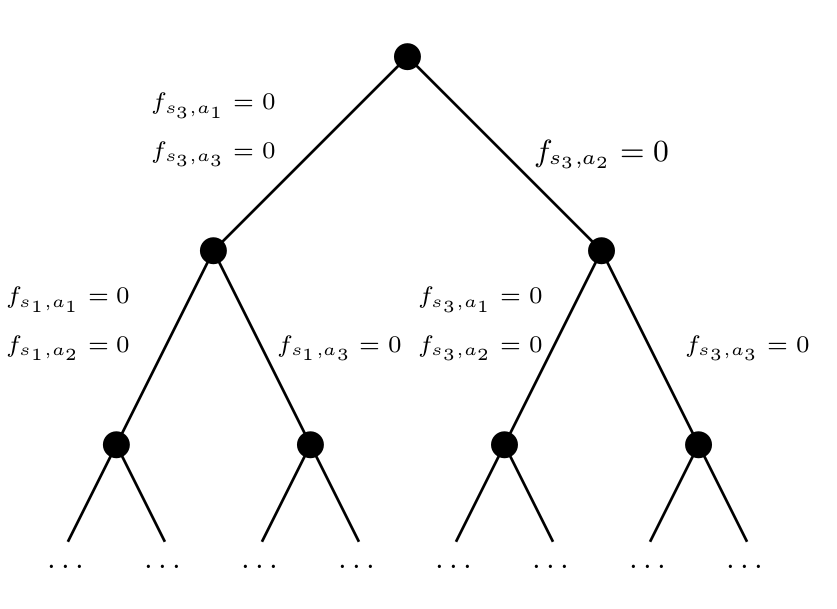
\includegraphics[scale=0.25]{images/bb.png}
	\end{center}
	\caption{Example of a branch-and-bound tree for an MDP with $4$ states and $3$ actions per state}
	\label{fig:pic_bb}
\end{figure}

%
%
%\begin{wrapfigure}{r}{0.6\textwidth}
%	\begin{center}
%    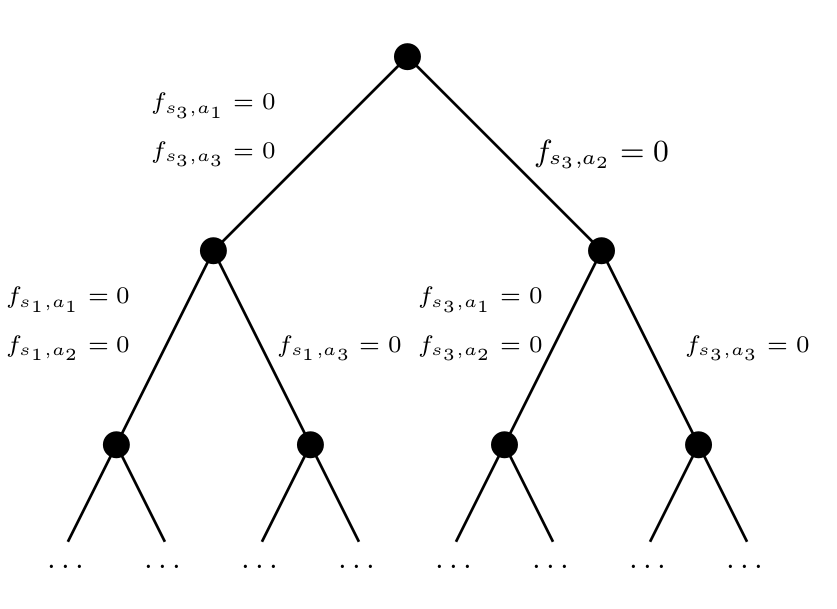
\includegraphics[scale=0.22]{images/bb.png}
%	\end{center}
%	\caption{Example of a branch-and-bound tree for an MDP with $4$ states and $3$ actions per state}
%	\label{fig:pic_bb}
%\end{wrapfigure}

%A branch-and-bound algorithm consists of a clever enumeration of the space of feasible policies through a space search: the set of deterministic policies that can potentially be the optimal is represented with a rooted tree with the full set associated to the root. The algorithm explores branches of this tree, where each branch represents a subset of the solution set.
%Once a new branch of the tree is created, and before that branches is split again in additional subbranches, a (lower) bounding procedure is executed on that branch. The bounding procedure gives an underestimation of the optimal solution of the problem over the feasible set associated to the given branch.
%The branch is hence discarded if it cannot produce a better solution than the best one found so far by the algorithm.

In our application, the root of the branch-and-bound tree is associated to the full set of deterministic policies, while a branch is obtained by selecting a couple $(s,a)$ of state and action and subsequently imposing the following disjunction on the two child nodes:
\begin{itemize}
\item $f_{s,a'}=0, \forall a'\neq a$ for the ``left'' child node.
\item $f_{s,a}=0$ for the ``right'' child node. 
\end{itemize} 
The disjunctions imposes to the left child to represent only deterministic policies with $f_{s,a}\neq 0$  (i.e. $\pi(s,a)=1$). On the other hand, the right child represents deterministic p with $f_{s,a}=0$  (i.e. $\pi(s,a)=0$)
\footnote{The total number of choices (i.e., the number of state-action pairs) is finite, therefore also the size of the branch-and-bond tree is finite.}. Figure~\ref{fig:pic_bb} presents an example of a branch-and-bound tree for an MDP with $4$ states and $3$ actions. 
%In this representation, we show at each node the additional restriction to the region 
 

%As already mentioned, 
To avoid exploring the whole tree, we need a lower bounding procedure to \textit{prune} some of the nodes that do not contain the optimal policy. In our application, we use the optimal stochastic policy as under-estimator of the optimal deterministic policy for a given branch of the tree (we remind that we are minimising, for this reason the underestimator can be viewed as an optimistic estimation of the policy). In this way, if a node has a stochastic policy higher than the best deterministic policy found so far it is not necessary to continue exploring that branch and the node can be pruned.

The final ingredient of a branch-and-bound is a procedure to find feasible deterministic policies. In our implementation, every time that a stochastic policy computed in the bounding procedures is also deterministic, its value can be used to update the value of the best known deterministic policy. %to its value.


In Figure~\ref{fig:basic_bb} we show the pseudo-code of our implementation of the branch-and-bound algorithm. The algorithm starts by initializing the value of the best known deterministic policy to $+\infty$ and the list of unexplored nodes to the root node (i.e., the one with no constraints on the $f$ variables).
The while loop extracts one unexplored node from the list, fixes the $f$ corresponding to its subregion of feasible deterministic policies and computes a lower bound with Benders decomposition. If the resulting optimal stochastic policy has a maximum regret $\delta^*$ greater or equal than the lower maximum regret found so far for a deterministic policy, no additional nodes are created and the loop extracts another node from the list. If the node is not pruned but the stochastic solution is deterministic, the value of the best deterministic solution is updated to $\delta^*$. As last option, if the stochastic solution is not deterministic, a state $s$ with more than one $f$ different from zero is found and the $f^*_{s,a}$ with the highest value is used to create the next two child nodes.

\textbf{Cut-and-branch version of the algorithm.}  %\label{sec:cb}
In the computational experiments, we test also a modification of the algorithm, called \textit{cut-and-branch}. In this version of the algorithm, we decide to solve the root note of the branch-and-bound tree as usual. % (i.e. with the standard interactin between master and slave). 
Once the algorithm starts to branch, additional Benders cuts are added only if the policy found by the the master problem is deterministic. In this way we are sure to compute correctly the value of the maximum regret of a deterministic solution. The advantage of the proposed approach is that the computing time needed to process a node is lower than the one needed by the basic version of the algorithm. On the other hand, the lower bounds obtained in the second case are weaker, this means that the total number of nodes explored can potentially be higher.
In the computation section we show how the cut-and-branch version of the algorithm outperforms the basic implementation.    



\begin{figure}[h!]
\noindent
\fbox{\hspace{\mylengthleft}\parbox[t]{\mylength}{\vspace*{0.5ex}
%
{\bf Algorithm } {\em } branch-and-bound search for an optimal deterministic policy:\\*[1ex]
%{\footnotesize // initialization}\\
$BestVal := +\infty$ {\em {\footnotesize /* best value fixed to infinity */}}\\
$\mathcal{N} = \{\{\emptyset\}\}$ {\em {\footnotesize /* the collection of open nodes is initialized with the empty set */}}\\
%{\bf for} $s := 0$ {\bf to} $C$ {\bf do}\\ 
%\hspace*{3ex} $f[s]=1$; $g[s]=1$\\*[1ex]
%{\em {\footnotesize consider one item at a time}}\\
{\bf while} $\mathcal{N}$ is not empty {\bf do}\\ 
\hspace*{3ex} extract node $N$ from $\mathcal{N}$\\
\hspace*{3ex} {\bf for each} $f$ {\bf in} $N$ {\bf do}:\\ 
\hspace*{3ex} \hspace*{3ex} fix $f=0$ in the master problem\\
\hspace*{3ex} solve the master problem with Benders decomposition\\
\hspace*{3ex} $(\delta^*,f^*) :=$ the optimal solution of the master problem\\
\hspace*{3ex} {\bf if} $\delta^* < Best Val$ {\bf then}: {\em {\footnotesize /* comparing the stoc. pol. with the best det. pol. */}}\\
\hspace*{3ex} \hspace*{3ex} {\bf if} $f^*$  is deterministic {\bf then}:\\
\hspace*{3ex} \hspace*{3ex} \hspace*{3ex} $BestVal = \delta^*$ {\em {\footnotesize /* update the best det. policy */}}\\
\hspace*{3ex} \hspace*{3ex} {\bf else}:\\
 \hspace*{3ex} \hspace*{3ex} \hspace*{3ex} {\em {\footnotesize /* create the two child nodes */}}\\
 \hspace*{3ex} \hspace*{3ex} \hspace*{3ex} find $f^*_{s,a}$ that correspond to a state that is not deterministic  \\
 \hspace*{3ex} \hspace*{3ex} \hspace*{3ex} $N_L := N \cup_{s' \neq s} f_{s',a}$  \\
\hspace*{3ex} \hspace*{3ex} \hspace*{3ex} $N_R := N \cup f_{s,a}$  \\
\hspace*{3ex} \hspace*{3ex} \hspace*{3ex} $\mathcal{N} := \mathcal{N} \cup N_L \cup N_R$\\
}}
\caption{Algorithm to find an optimal deterministic policy.} \label{fig:basic_bb}
\end{figure}


\section{Theoretical analysis of the optimal deterministic policy}\label{sec:comparison}

%
%\begin{wrapfigure}{r}{0.5\textwidth}
%	\begin{center}
%    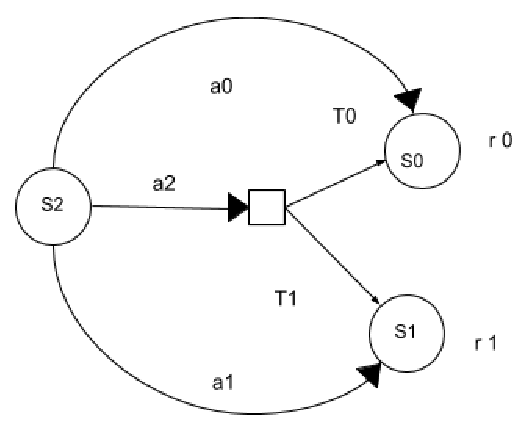
\includegraphics[scale=0.4]{images/Trident_MDP.pdf}
%	\end{center}
%	\caption{Trident IRMDP with $3$ states and $3$ actions.}
%	\label{fig:trident} 
%\end{wrapfigure}

In this section we first introduce the intuitive concept of rounding heuristic, a way to obtain a feasible deterministic policy starting from a stochastic optimal policy. Subsequently, we analyse the situations where such rounding heuristic could provide maximum regrets far from the one given by the optimal deterministic policy.

\paragraph{\textbf{The ``rounding'' heuristic.}}%\label{sec:rounding}

Let $\tilde{f}$ be a given visitation frequency value for the optimal stochastic policy. The corresponding ``rounding'' deterministic policy $\hat{\pi}$ can be computed as follows:

\begin{itemize}
\item for each $s'\in S$:
\begin{itemize}
\item find the action $a' = \text{argmax}_{a \in A}f_{s',a}$.
\item fix the rest of the action to zero: $\hat{f}_{s',a} =0, \forall a \neq a'$
\end{itemize}
\item recover the deterministic policy $\hat{\pi}$ obtained from the above fixing.
\end{itemize} 
 
The heuristic approach computes the deterministic policy by selecting the action with the highest probability for each state. Despite being pretty simple, this approach represents a plausible behaviour of a user that want to derive a deterministic policy starting from a stochastic one. 
%
%For the \textit{Tiny MDP} presented in Bruno's manuscript, it is easy to check that the rounding heuristic always gives the optimal deterministic policy (i.e., the one that minimises the max regrets).
%
%What we would like to find is a class of instances where this is not the case or, even better, instances where the difference between the heuristic deterministic policy and the optimal deterministic policy can be arbitr
%
%For a given node of the branch and 
%As bounding procedure   
%
%All the tests so far showed that the vast majority of the benders inequalities are added in the computation of the root node of the branch-and-bound (i.e., in the computation of the stochastic policy), we hope that in this way the time spent in the enumeration of the branch-and-bound tree will be reasonable.
%

\paragraph{\textbf{A small counterexample.}}%\label{sec:counter}

We define the \textit{Trident IRMDP} (see Figure~\ref{fig:trident}) as follows:
\begin{itemize}
\item Three states: $s_0, s_1, s_2$, three actions $a_0, a_1, a_2$ and a discout factor $\gamma=1$.
\item A transition function: $P(s_0 | s_2,a_0)=1$, $P(s_1 |s_2 ,a_1)=1$, $P(s_0 | s_2, a_2) = T_0$ and $P(s_1 | s_0, a_2) = T_1$.\footnote{in this formulation rewards are dependent on states. They can be easily modified to the reward function notation given in this paper $r(s, a)$} 	 
\item Two unknown rewards associated to $s_0$ and $s_1$: $r(a_0)= r_0 \in [-A,+A]$ and $r(a_1)= r_1 \in [-A+B,+A+B]$ with $A,B > 0$ and $A \gg B$. Thus, $\mathcal{R} = [-A, +A]\times[-A+B, A+B]$
\item An initial distribution on states $\beta(s_0)= \beta(s_1) = 0$ and $\beta(s_2)=1$.

\end{itemize} 

%%%%%%%%%%%%%%%%%
\begin{figure}[]
	\begin{center}
    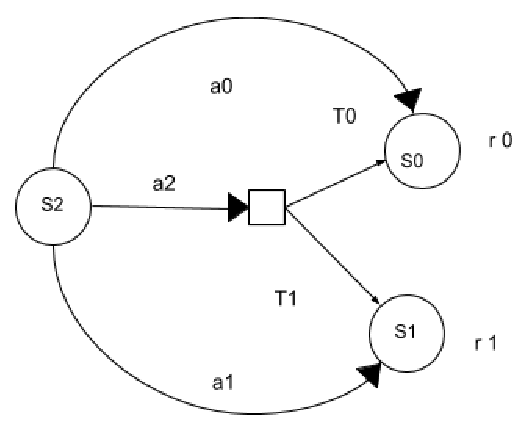
\includegraphics[scale=0.4]{images/Trident_MDP.pdf}
	\end{center}
	\caption{Trident IRMDP with $3$ states and $3$ actions.}
	\label{fig:trident} 
\end{figure}
%%%%%%%%%%%%%%%%%

The following propositions give a complete characterization of the optimal stochastic and deterministic policies for the Trident MDP. With a slight abuse of notation, we use the pedix $a$ instead of using $s_2,s_a$, i.e. instead of writing $\pi(s_2, s_a)$ we use $\pi_a$. 
%According to Figure~\ref{fig:trident}, this is due to the fact that two states $s_0$ and $s_1$ are terminal states and the only relevant actions are the ones originating from the state $s_2$ (for example, we use $\pi_1$ instead of $\pi(s_2, a_1)$). 
%For the same reason, 
We also use $r_{0}$ in place of $r(s_0)$ and $r_{1}$ in place of $r(s_1)$. Each stochastic policy on the trident MDP can be demonstrated as a tuple $\pi = (\pi_0, \pi_1, \pi_2)$. %where each element indicates the probability of choosing action $a_i$ in state $s_i$. 
Similarly, the visitation frequency functions are presented as $f = (f_0, f_1, f_2)$.

\begin{proposition}\label{theorem:opt_stoc}
An optimal stochastic policy that minimises the maximum regret (see Section~\ref{sec:Preliminaries}) for the Trident MDP is the policy $\tilde{\pi} = (\pi_0, \pi_1, \pi_2)$ defined as:
$$\pi_{0}=\dfrac{2A - B}{4A},~~~\pi_{1}=\dfrac{2A + B}{4A}, ~~~\pi_2 = 0\;.$$
%(regardless of the values of $T_1$ and $T_2$). \footnote{We recall that $\pi_0$ means $\pi(s_2, a_0)$ and so on.}
\end{proposition}
\begin{proof}
%We first show that there exists always an optimal stochastic policy with $\pi_2 = 0$. We do this by
We first observe that for every policy $\pi' = (\pi'_0, \pi'_1, \pi'_2)$ with $\pi'_2 > 0$, it is possible to construct a policy $\pi'' = (\pi''_0, \pi''_1, \pi''_2)$ with $\pi''_2 = 0$ and with the same value in the following way:
\vspace{-0.2cm}
\begin{align*}
\pi''_0 = \pi'_0 + \pi'_2 T_0, ~~~ \pi''_1 = \pi'_1 + \pi'_2 T_1\;.
\end{align*}
If we compute the value of the first policy we notice that:
\vspace{-0.2cm}
\begin{align*}
\beta \cdot V^{\pi'} = V^{\pi'}(s_2) =
r_{_0} \pi'_0 + r_{_1}\pi'_1 + r_{_0} T_0 \pi'_2 + r_{_1} T_1 \pi'_2 \\
= r_{_0} (\pi'_0 + T_0 \pi'_2) + r_{_1} (\pi'_1 + T_1 \pi'_2)
= r_{_0} \pi''_0 + r_{_1}\pi''_1 = V^{\pi''}(s_2) =\beta \cdot V^{\pi''}\;,
\end{align*}
showing that both policies have the same value.
\ET{Moreover, the equivalence shows that  $\beta \cdot V^{\pi'}= \beta \cdot V^{\pi''}$, $\forall r \in \mathcal{R}$,
this implies that
$\pi'$ and $\pi''$ have equivalent maximum regret, because: $MR(\pi', \mathcal{R}) = \text{max}_{r} \text{max}_g r \cdot g - \beta \cdot V^{\pi'} = \text{max}_{r} \text{max}_g r \cdot g - \beta \cdot V^{\pi''} = MR(\pi'', \mathcal{R})$.}
% indicates that for each stochastic policy there exists a stochastic policy with the same value but with $\pi_2 = 0$. 
We can hence suppose that there exists an optimal stochastic policy with $\pi_2 =0$ as a solution for minimax regret. 

As second part of the proof, we compute the value of the optimal policy considering $\tilde{\pi} = (\pi_0, \pi_1, 0)$ where $\pi_0, \pi_1 \geq 0$ similarly its equivalent visitation frequency is $\tilde{f} = (f_0, f_1, 0)$. 
%Let $\pi_0,\pi_1$ be a generic policy. 
We notice that the adversary policy by its equivalent visitation frequency $g$ giving a maximum regret is always deterministic (see~\ref{sec:Preliminaries}). For this reason, we have only two adversary policies: we can have either $g = (g_0, g_1, g_2)$ where $g_0 = g_2=0$ and $g_1 > 0$ or the opposite, $g' = (g_0, g_1, g_2)$ where $g_0>0$ and $g_1 = g_2 = 0$. (We notice that, with arguments analogous to the ones used in the first part of the proof, we can rule out the case where $g_2 \geq 0$.)

Knowing that the maximum regret is the maximum among two choices for the adversary policies, the maximum regret associated to the policy $g =(0, g_1, 0)$ (obtained by fixing $r_0 = -A$ and $r_1 = A+B$) is the following
\vspace{-0.2cm}
\begin{align}
r \cdot g - r \cdot \tilde{f} = A + B +A \pi_0 -(A+B)\pi_1 \label{eq:best_stoc_1}
\end{align}   
and the maximum regret associated to the policy $g' = (g_0, 0, 0)$ where $g_0 > 0$ is obtained by fixing $r_0 = A$ and $r_1 = -A+B$, leading to a value of
\vspace{-0.2cm}
\begin{align}
r \cdot g - r \cdot \tilde{f}  = A - A \pi_0 -(B-A)\pi_1 \label{eq:best_stoc_2}\;.
\end{align}   
We are interested in minimising the max regret, this means that we want to find the values of $\pi_0$ and $\pi_1$ that minimise $\max \{\eqref{eq:best_stoc_1}, \eqref{eq:best_stoc_2}\}$. The optimal stochastic policy can hence be obtained by solving the following system of two equations: 
\vspace{-0.2cm}
\begin{align*}
A + B +A \pi_0 -(A+B)\pi_1 &= A - A \pi_0 -(B-A)\pi_1\\
\pi_0+\pi_1 &= 1
\end{align*} 
That has as optimal solution the values $\pi_{0}=\dfrac{2A - B}{4A}$ and $\pi_{1}=\dfrac{2A + B}{4A}$, concluding the proof.$\square$
\end{proof}


Proposition~\ref{theorem:opt_stoc} implies the following Lemma:
\begin{lemma}\label{lemma:heur_policy}
The rounding deterministic policy for the Trident MDP is $\hat{\pi} = (0, 1, 0)$ %$ $\pi_0 =\pi_2 = 0$ and $\pi_1 = 1$ 
and its maximum regret is $MR(\hat{f}, \mathcal{R}) = 2A-B$.
\end{lemma}
\begin{proof}
It is a direct consequence of the fact that in the optimal stochastic policy we always have $\pi_1 > \pi_2$ and $\pi_0 = 0$.$\square$
\end{proof}

\begin{proposition}\label{theorem:opt_det}
If $T_1 > T_0$, the optimal deterministic policy is $\pi^* = (0, 0, 1)$ and its maximum regret is $MR(f^*, \mathcal{R}) = A- A T_0 +(A-B) T_1$. 
\end{proposition}
\begin{proof}
We prove the statement by explicitly computing the maximum regret of the three possible deterministic policies:$\pi = (1, 0, 0), \pi' =(0, 1, 0), \pi''= (0, 0, 1)$ $\pi_0=1$.

\textit{Maximum regret of $\pi = (1, 0, 0)$}. We want to find the adversary policy that maximises the regret for the policy $\pi$. We do that by computing all possible combinations of adversary policies and rewards:
\begin{itemize}
\item If a visitation frequency for adversary policy is $g = (0, g_1, 0)$ where $g_1> 0$, the reward maximising the regret is $r_0 = -A$ and $r_1 = A+B$, leading to a maximum regret of 
\vspace{-0.5cm}
\begin{align}
A+B-(-A)=2A+B \label{eq:regret0}
\end{align}
\item If the adversary policy is $g' = (0, 0, g_2)$ where $g_2>0$, we need to check all four combinations of extreme rewards:
\begin{itemize}
\item $r_0 = -A$ and $r_1= A+B$. Maximum regret of
\vspace{-0.2cm}
\begin{align}
-A T_0 + (A+B)T_1 + A = (1-T_0 + T_1)A + T_1 B \label{eq:regret1}
\end{align}
\item $r_0 = A$ and $r_1= A+B$. Maximum regret of
\vspace{-0.2cm}
\begin{align}
A T_0 + (A+B)T_1 - A = (-1+T_0 + T_1)A + T_1 B  \label{eq:regret2}
\end{align}
\item $r_0 = A$ and $r_1= -A+B$. Maximum regret of
\vspace{-0.2cm}
\begin{align} 
A T_0 + (-A+B)T_1 - A =  (-1+T_0 - T_1)A + T_1 B \label{eq:regret3}
\end{align}
\item $r_0 = -A$ and $r_1= -A+B$. Maximum regret of
\vspace{-0.2cm}
\begin{align}
-A T_0 + (-A+B)T_1 + A =  (1 - T_0 - T_1)A - T_1 B \label{eq:regret4}
\end{align}
\end{itemize} 
By hypothesis we have that $A\gg B$ and $T_0+T_1= 1$, this implies that $\eqref{eq:regret0} \geq \max\{\eqref{eq:regret1}, \eqref{eq:regret2}, \eqref{eq:regret3}, \eqref{eq:regret4} \}$. Therefore, the maximum regret if $g_2>0$ is $MR(f^{\pi}, \mathcal{R}) = 2A+B$.
\end{itemize} 

\textit{Maximum regret of $\pi' = (0, 1, 0)$}.
It is trivial to check, with calculations analogous to the one used above to compute the regret of $\pi$, that the maximum regret in this case is equal to $MR(f^{\pi'}, \mathcal{R}) = 2A-B$.


\textit{Maximum regret of $\pi'' = (0, 0, 1)$}.
Also in this case, we need to consider the two cases of $g =(g_0, 0 ,0)$ where $g_0 > 0$ and $g' = (0, g_1, 0)$ with $g_1 > 0$. For $g$, we fix $r_0 = A$ and $r_1 = -A+B$, obtaining a regret equal to 
\vspace{-0.2cm}
\begin{align}
A- A T_0 +(A-B) T_1 \label{eq:regret2_1}
\end{align}
And for $g'$ we fix $r_0 = -A$ and $r_1 = A+B$, obtaining a regret equal to 
\vspace{-0.2cm}
\begin{align}
A+B+A T_0 -(A+B) T_1\;. \label{eq:regret2_2}
\end{align}
The maximum between~\eqref{eq:regret2_1} and~\eqref{eq:regret2_2} depends on the values of $T_0$ and $T_1$.
By imposing  $A- A T_0 +(A-B) T_1 \geq A+B+A T_0 -(A+B) T_1$ we obtain:
$$ 2A T_1 \geq 2 A T_0 + B\;. $$
We recall that by construction we have $A \gg B$, this implies that if $T_1> T_0$ (resp. $T_1\leq T_0$)  we have that the maximum regret is equal to~\eqref{eq:regret2_1} (resp.~\eqref{eq:regret2_2}).
The minimum maximum regret found so far is the one obtained for $\pi = \pi' = (0, 1, 0)$, and it is equal to $MR(f^{\pi'}, \mathcal{R}) = 2A-B$. Therefore, it remains to check for which values of $T_0 > T_1$ we have that $2A-B \geq~\eqref{eq:regret2_1}$:
\vspace{-0.2cm}
\begin{align*}
A- A T_0 +(A-B) T_1 \leq 2A - B \Leftrightarrow A- A (1-T_1) +(A-B) T_1 \leq 2A - B\\
  \Leftrightarrow (2A-B)T_1 \leq 2A-B  \Leftrightarrow T1 \leq 1\;.
\end{align*}
 Since we have by construction that $T_1 \leq1$ we can conclude that for any $T_1> T_0$ the optimal deterministic policy is $\piç* = \pi''= (0, 0,1)$ and its maximum regret is equal to $MR(f^{\pi''}, \mathcal{R})A- A T_0 +(A-B) T_1$. $\square$
\end{proof}

Proposition~\ref{theorem:opt_det} and Lemma~\ref{lemma:heur_policy} shows that for any Trident MDP we have that the optimal deterministic policy and the rounding deterministic policy are always different. 


The following Lemma shows that the rounding policy could be significantly worse than the optimal deterministic policy:

\begin{lemma}\label{lemma:gap2}
The ratio between the maximum regret of the rounding deterministic policy and the optimal deterministic policy goes to $2$ with the increase of the value of $A$ with respect to $B$ and the increase of $T_1$. In other words:  
\vspace{-0.2cm}
\begin{align*}
\lim_{A/B \rightarrow \infty, T_1 \rightarrow {\frac{1}{2}}^+} \dfrac{2A-B}{A- A T_0 +(A-B) T_1} = 2
\end{align*}
\end{lemma}
\begin{proof}
The statement follows from the definition of the limit.$\square$
\end{proof}

%Lemma~\ref{lemma:gap2} shows that even small MDP can present

From a theoretical point of view, it is still unknown if some MDPs can have a ratio greater than $2$ (or even a ratio that goes to infinity). From a practical point of view, such small example shows how the use of the rounding policy can lead to a maximum regret  $100\%$ far from the optimal. 

\section{Experimental results}\label{sec:experiments}

In this section, we provide an experimental evaluation of our approach
based on two classes of test instances. More precisely, we test our approach on the following MDPS:
\begin{itemize}
\item Random MDPs (\texttt{Random}).
\item Diamond MDPs (\texttt{Diamond}).
\item Grid MDPs (\texttt{Grid}).
\end{itemize}


For each class of MDP, we provide a brief description of its structure and of the parameters used to generate the testbed.

As already mentioned in the introduction, the aim of this section is two-fold:

(i) First of all, we would like to motivate the use of deterministic over stochastic policies. To do this, we compare the value of the maximum regret obtained by the optimal deterministic policy with the one of the rounding policy explained in Section~\ref{sec:rounding}. 
%
%The TUP uses the concept of sparsity presented in this paper to generalize the methodology proposed in~\cite{Buchheim18} to solve efficiently combinatorial problems with a quadratic objective function.
%In Section~\ref{sec:TUP} we show how the application of TUD allows to improve the dual bounds obtained in the approach presented in~\cite{Buchheim18}.  

(ii) Secondly, we would like to assess the additional computational effort of computing the optimal deterministic policy in comparison to the one needed to compute the optimal stochastic policy. 	 

In the following section we use the notion of Time ratio ($TR$) and Value Ratio ($VR$), defined as follows:

\begin{definition}
For a given MDP, let $MR(f^{\hat{\pi}}, \mathcal{R})$ be the maximum regret of the rounding deterministic policy and $MR(f^{\pi^*}, \mathcal{R})$  be the maximum regret of the optimal deterministic policy. We have that the Value Ratio of such MDPs is defined as follows:
\begin{align}
VR = \dfrac{MR(f^{\hat{\pi}}, \mathcal{R})}{MR(f^{\pi^*}, \mathcal{R})}\;.
\end{align} 
Moreover, let $\hat{T}$ (respectively $T^*$) be the computing time necessary to calculate the rounding (respectively optimal) deterministic policy, we have that the Time Ratio is defined as:
\begin{align}
TR=\dfrac{T^*}{\hat{T}}\;.
\end{align}
 
\end{definition}

\subsection{Random MDPs}
\paragraph{Description}
A random MDP is defined by several parameters including its number of states $n$ , its number of actions $k$. All rewards are bounded between randomly two real numerical points. Transition function has several properties: from any state $s$ restrict transitions to reach $\lceil \log_2(n) \rceil$ states. For each pair of $(s, a)$ draw reachable states based on uniform
distribution over the set of states. For drawn states, transition probabilities are formed based on Gaussian distribution.
The initial state distribution β is uniform and we choose discount factor $\gamma = 0.95$. 
\paragraph{Analysis of the results}
In Table~\ref{tab:random} we have th resutm

\begin{table}[h] % <-- HERE
 \setlength{\tabcolsep}{2.5pt}
 \renewcommand \arraystretch{1.1}
\begin{center}
\begin{tabular}{rrrrrrrrrrrrrrrrrrrrrrrrrrrr}
	&		&				&				&				&	\multicolumn{2}{c}{	\texttt{Comp. Time}}	\\
$|S|$	&	$|A|$	&		\texttt{VR}		&		\texttt{TR}		&		\texttt{\% diff}		&	\texttt{Base}	&	\texttt{C\&B}	\\
\cmidrule(lr){1-2} \cmidrule(lr){3-3} \cmidrule(lr){4-4}  \cmidrule(lr){5-5}  \cmidrule(lr){6-7}
5	&	2	&			1.07	&			1.83	&			50\%	&	2.59	&	2.27	\\
	&	3	&			1.03	&			2.44	&			20\%	&	5.05	&	5.11	\\
	&	4	&			1.09	&			2.17	&			50\%	&	5.28	&	4.67	\\
	&	5	&			1.07	&			2.85	&			50\%	&	8.03	&	7.99	\\
	&	10	&			1.02	&			2.50	&			30\%	&	13.76	&	12.61	\\
\cmidrule(lr){1-2} \cmidrule(lr){3-3} \cmidrule(lr){4-4}  \cmidrule(lr){5-5}  \cmidrule(lr){6-7}
10	&	2	&			1.11	&			4.11	&			90\%	&	21.78	&	20.12	\\
	&	3	&			1.15	&			7.63	&			80\%	&	81.67	&	73.43	\\
	&	4	&			1.04	&			9.19	&			60\%	&	312.05	&	266.35	\\
	&	5	&			1.06	&			8.42	&			90\%	&	570.15	&	478.07	\\
	&	10	&			1.01	&			18.79	&			90\%	&	1886.05	&	986.71	\\
\cmidrule(lr){1-2} \cmidrule(lr){3-3} \cmidrule(lr){4-4}  \cmidrule(lr){5-5}  \cmidrule(lr){6-7}
15	&	2	&			1.04	&			6.91	&			60\%	&	94.95	&	82.59	\\
	&	3	&			1.05	&			18.75	&			80\%	&	2240.40	&	2024.85	\\
	&	4	&			1.01	&			20.04	&			80\%	&	5366.92	&	3181.01	\\
	&	5	&			1.03	&			32.10	&			100\%	&	7677.25	&	4127.52	\\
\cmidrule(lr){1-2} \cmidrule(lr){3-3} \cmidrule(lr){4-4}  \cmidrule(lr){5-5}  \cmidrule(lr){6-7}
	&	Avg.	&			1.06	&			7.77	&			70\%	&	1306.14	&	805.24	
\end{tabular}						
\end{center}
\caption{Time Ratio and Value Ratio for \texttt{Random} MDPs.}														\label{tab:random}								
\end{table} % <-- HERE



\subsection{Diamond MDPs}
\paragraph{Description}
This class of MDPs has been introduced for the first time in~\cite{benavent2018}. 
In this family of problems the reward of a few states suffices to generate a lot of uncertainty about the optimal policy. This class of instances is an interesting set of instancess to test our proposed algorithm.
This class of MDPs has a diamond structure, with one top and one bottom state (playing the role of source and sink of the  MDP), one intermediate layer of states, containing all the uncertainty in the reward, plus two intermediate layer between the extrem states and the intermediate layer.
In Figure~\ref{fig:diamond}, the structure of the diamond MDPs is presented.

\begin{figure}[h]
\begin{center}
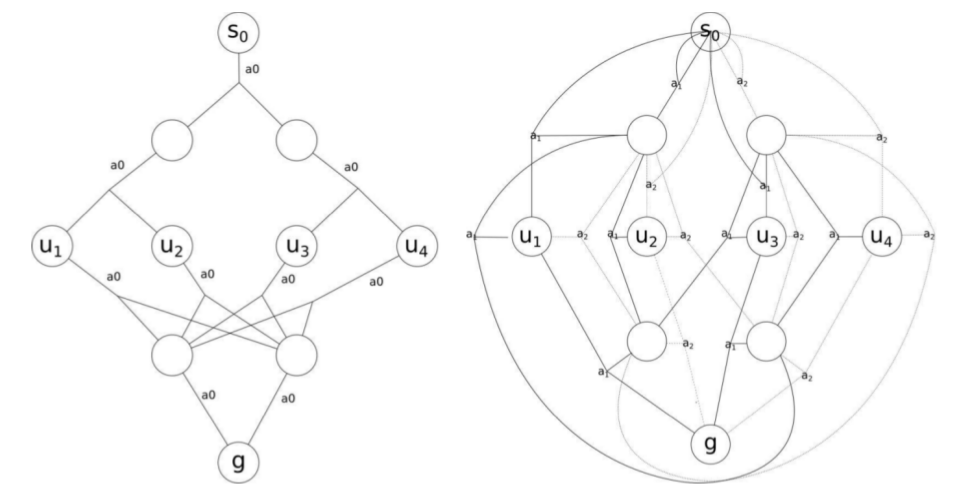
\includegraphics[width=8cm]{images/diamond.png}
\end{center}
\caption{Diamond MDP: actions $a_0$ (left) and $a_1, a_2$ (right).}
\label{fig:diamond}
\end{figure}

From a point of viex of the parameters, the authors proposed to have that action $a_0$ would reach each child with a probability of $0.5$. ON the other hand $a_1$ (resp. $a_2$) a probability of $p= 0.3$ (resp. $1-0.3$) to reach the left (resp. right) child node and to reach its parent otherwise.
The imprecise values of the rewards for the middle layer are $[-600,600]$, while the one of the bottom node is $[600,1000]$.

We propose a generalization of this family of MDP in two senses: we test a range of parameters for the probability $p \in \{5,10,\dots,40,45\}$ and we introduce also an additional intermediate layer, between the extreme states and the middle layer. In this way we have, in addition to $10$-states MDPs (callend one-level diamond MDPs) also  22-states MDPs (called two-level diamond MDPs). 

\paragraph{Analysis of the results}
In Table~\ref{tab:diamond} We show


\begin{table}[h]																	
 \centering
 \small
 \setlength{\tabcolsep}{4.0pt}
 \renewcommand \arraystretch{1.8}
\begin{tabular}{ccccccccccc}																						
p	&	5	&	10	&	15	&	20	&	25	&	30	&	35	&	40	&	45	&	Avg.	\\	
\cmidrule(lr){1-1} \cmidrule(lr){2-10} \cmidrule(lr){11-11}
VR &	1.66	&	1.24	&	1.16	&	1.13	&	1.15	&	1.15	&	1.15	&	1.14	&	1.16	&	\textbf{1.22}	\\	
TR &	10.23	&	7.44	&	6.32	&	6.48	&	7.67	&	5.93	&	7.62	&	10.46	&	13.80	&	\textbf{8.44}	\\	\\
\end{tabular}
\caption{Time Ratio and Value Ratio for \texttt{Diamond}.}														\label{tab:diamond}								
\end{table}																						



\subsection{Grid MDPs}
blablabla
\paragraph{Description}
blablabla
\paragraph{Analysis of the results}
blablabla



\paragraph{Analysis of the Diamond MDPs}



\section{Conclusions}
We presented an algorithm to find an optimal deterministic policy that minimises the maximum regret of a Markov Decision Processes (MDP) with imprecise rewards.
The proposed algorithm consists of a branch-and-bound that uses Benders decomposition as bounding procedure. %In addition to a basic implementation, we propose a cut-and-branch implementation that turns out to reduce the overall computing time on average by $50\%$.  
We motivate the use of deterministic over stochastic policies by showing that basic rounding procedures find deterministic policies far from the optimal. Secondly, we show that the additional computational effort of computing the optimal deterministic policy in comparison to the one needed to compute the optimal stochastic policy is acceptable (approximately one order of magnitude slower).
%We hope that this manuscript motivates the scientific community to investigate more the development of algorithm for deterministic solutions in the context of MDPs with imprecise rewards. 
		




%%%%%%%%%%%%%%%%%%%%%%%%%%%%%%%%%%%%%%%%%%%%%%%%%%%%%%%%%%%%%%%%%%%%%%%%%%%%%%%%%%%%%%%%%%%%%%%%%%%%%%%%%
%% bibliography: see CFP for number of permitted pages

\bibliographystyle{ACM-Reference-Format}
\bibliography{biblio}

\end{document}
